%!TEX root = ../../super_main.tex

\section{Launcher}
The \giraf-\launcher is a specialized Android launcher application which is be used to populate the home screen of an Android device. Most Android devices come bundled with a default launcher for their home screen and most users never think to replace it. An Android launcher is the main entry point, for users, to the graphical user interface for Android. Launchers are used to make other installed applications available to the user, usually done through a grid of Android applications and widgets. The intended purpose of the \giraf-\launcher, besides the functionality of a regular launcher, is to give the user a single entrance to the \giraf software suite and to give the illusion of using the \giraf-system and not Android. A screenshot of the initial \androidinline{HomeActivity} of the \launcher can be seen in \figref{fig:initial_launcher}. \todo{DONE-start}The \launcher should is used a customizable filter for the citizens, such that the citizens only is shown applications they can use. This filter is maintained by the guardian. However, a the \launcher allows for showing all applications installed on the device, including non-\giraf applications. \todo{DONE-end}
\\\\
The \launcher project also contains the login and authentication part of the \giraf suite, which a user has to pass through before being able to use the \launcher itself. The authentication system is being developed by another group in the first sprint, and will therefore not be considered in this part of this report. 

\begin{figure}[!htbp]
	\centering
	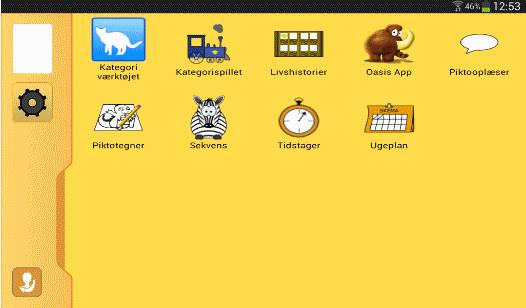
\includegraphics[width=\textwidth]{sprint_one/initial_launcher}
	\caption{Initial Launcher}
	\label{fig:initial_launcher}
\end{figure}
